% =====================================================================
% Plan de tesis FDTooth — formato de "PLAN DE TESIS (2).docx" (ESAN)
% A4, márgenes 2.54 cm, Times New Roman 12, interlineado doble,
% justificado, sangría de primera línea 1.25 cm, referencias APA 7.
% Compilar: latexmk -pdf main.tex   (pdflatex + biber)
% =====================================================================
\documentclass[12pt,a4paper]{article}

\usepackage[T1]{fontenc}
\usepackage[utf8]{inputenc}
\usepackage[spanish,es-tabla,es-nodecimaldot]{babel}
\usepackage{newtxtext,newtxmath}
\usepackage[a4paper,margin=2.54cm]{geometry}
\usepackage{setspace}
\usepackage{graphicx}
\usepackage{booktabs,tabularx,array}
\usepackage{titlesec}
\usepackage[labelfont=bf,labelsep=period]{caption}
\usepackage{csquotes}
\usepackage[style=apa,backend=biber]{biblatex}
\usepackage[hidelinks]{hyperref}
\usepackage{xcolor}
\addbibresource{referencias.bib}
\graphicspath{{img/}}

% ---- Código de colores de redacción (guías del curso) -----------------
% \prob{} problema (VD) = azul   | \sol{} solución/técnica (VI) = rojo
% \dat{}  dataset/datos  = verde  | \con{} conector de adición = resaltado
% Para la versión final cambia \colorestrue por \coloresfalse.
\definecolor{problema}{RGB}{0,112,192}
\definecolor{solucion}{RGB}{192,0,0}
\definecolor{dataset}{RGB}{0,128,0}
\newif\ifcolores
\colorestrue
\ifcolores
  \newcommand{\prob}[1]{\textcolor{problema}{\textbf{#1}}}
  \newcommand{\sol}[1]{\textcolor{solucion}{\textbf{#1}}}
  \newcommand{\dat}[1]{\textcolor{dataset}{\textbf{#1}}}
  \newcommand{\con}[1]{{\setlength{\fboxsep}{0.5pt}\colorbox{yellow}{\strut #1}}}
\else
  \newcommand{\prob}[1]{#1}
  \newcommand{\sol}[1]{#1}
  \newcommand{\dat}[1]{#1}
  \newcommand{\con}[1]{#1}
\fi

\doublespacing
\setlength{\parindent}{1.25cm}

% ---- Títulos: todos 12 pt negrita; capítulos centrados -----------------
\setcounter{secnumdepth}{4}
\renewcommand{\thesection}{\Roman{section}}
\renewcommand{\thesubsection}{\arabic{section}.\arabic{subsection}.}
\renewcommand{\thesubsubsection}{\arabic{section}.\arabic{subsection}.\arabic{subsubsection}.}
\renewcommand{\theparagraph}{\thesubsubsection\arabic{paragraph}.}
\titleformat{\section}{\normalfont\bfseries\centering}{CAPÍTULO \thesection:}{0.4em}{}
\titleformat{\subsection}{\normalfont\bfseries}{\thesubsection}{0.5em}{}
\titleformat{\subsubsection}{\normalfont\bfseries}{\thesubsubsection}{0.5em}{}
\titleformat{\paragraph}[hang]{\normalfont\bfseries}{\theparagraph}{0.5em}{}
\titlespacing*{\paragraph}{0pt}{1ex}{0.5ex}
% Secciones sin número (Introducción, Referencias, Anexos), centradas
\newcommand{\seccionsinnumero}[1]{%
  \section*{#1}\addcontentsline{toc}{section}{#1}}

\begin{document}

% ======================= CARÁTULA ====================================
\begin{titlepage}
\centering
\onehalfspacing
\vspace*{1cm}
{\bfseries UNIVERSIDAD ESAN\par}
{\bfseries FACULTAD DE INGENIERÍA\par}
{\bfseries INGENIERÍA DE TECNOLOGÍAS DE INFORMACIÓN Y SISTEMAS\par}
\vspace{3cm}
% Título definitivo (patrón PREDICTIVO_TEMAS):
% Diseño de un Sistema de [SOLUCIÓN] para el Pre-diagnóstico de [PROBLEMA]
% a partir de [DATOS]
{\bfseries Diseño de un Sistema de \sol{Visión Computacional} para el
Pre-diagnóstico de \prob{Fenestración y Dehiscencia Ósea Alveolar} a partir
de \dat{Fotografías Intraorales y Tomografías CBCT}\par}
\vspace{1.5cm}
Plan de tesis\par
\vspace{2cm}
José Cabrera Ticlla\par
Lucero Ayala Mauricio\par
\vspace{1cm}
Asesor: Wilfredo Mamani Ticona\par
\vfill
Lima, diciembre de 2026\par
\end{titlepage}

% ======================= PRELIMINARES ================================
\pagenumbering{roman}

\begin{flushright}
\onehalfspacing
\textbf{DEDICATORIA}\par
\vspace{1cm}
\textit{Dedicatoria.}
\end{flushright}
\clearpage

{\onehalfspacing
\renewcommand{\contentsname}{Índice}
\tableofcontents
\clearpage
\renewcommand{\listfigurename}{Índice de Figuras}
\listoffigures
\renewcommand{\listtablename}{Índice de Tablas}
\listoftables
\clearpage}

\begin{center}\textbf{Resumen}\end{center}
% Estructura: introducción (8 líneas). "El objetivo de la presente
% investigación es <OG>" (6 líneas). Metodología (8 líneas). Resultados
% principales (5 líneas). Conclusiones principales (7 líneas).
Por redactar.

\noindent\textbf{Palabras clave:} \prob{fenestración}, \prob{dehiscencia},
\dat{CBCT}, \dat{fotografía intraoral}, \sol{Deep Learning},
\sol{Machine Learning}.

\begin{center}\textbf{Abstract}\end{center}
To be written.

\noindent\textbf{Keywords:} \prob{fenestration}, \prob{dehiscence},
\dat{CBCT}, \dat{intraoral photography}, \sol{Deep Learning},
\sol{Machine Learning}.
\clearpage

\ifcolores
\noindent\fbox{\parbox{\dimexpr\linewidth-2\fboxsep-2\fboxrule}{\small
\textbf{Borrador.} \prob{Problema} \quad \sol{Solución} \quad
\dat{Dataset} \quad \con{Del mismo modo, Asimismo, Por otra parte}}}
\fi

% ======================= CUERPO =====================================
\pagenumbering{arabic}

\seccionsinnumero{Introducción}
% Unas 2 páginas. Mismo embudo que el paper: mundo -> región -> Perú ->
% IA como respuesta. Ver ../Paper_FDTOOH/GUIA_REDACCION_PAPER.md
Por redactar.

% ---------------------------------------------------------------------
\section{Planteamiento del Problema}
Por redactar.

\subsection{Descripción de la Realidad Problemática}
Por redactar.

\subsection{Formulación del Problema}
Para la identificación del problema general y de los problemas específicos
\ldots

\subsubsection{Problema general}
¿\ldots?

\subsubsection{Problemas específicos}
% Uno por fase de la metodología (Fase 1..N).
\begin{description}
  \item[PE1:] ¿\ldots?
  \item[PE2:] ¿\ldots?
  \item[PE3:] ¿\ldots?
  \item[PE4:] ¿\ldots?
\end{description}

\subsection{Objetivos de la Investigación}
Para la identificación del objetivo general y de los objetivos específicos
\ldots

\subsubsection{Objetivo general}
Implementar \ldots

\subsubsection{Objetivos específicos}
\begin{description}
  \item[OE1:] \ldots
  \item[OE2:] \ldots
  \item[OE3:] \ldots
  \item[OE4:] \ldots
\end{description}

\subsection{Justificación de la Investigación}
\subsubsection{Teórica}
Por redactar.
\subsubsection{Práctica}
Por redactar.
\subsubsection{Metodológica}
Por redactar.

\subsection{Delimitación del Estudio}
\subsubsection{Espacial}
Por redactar.
\subsubsection{Temporal}
Por redactar.
\subsubsection{Conceptual}
Por redactar.

% ---------------------------------------------------------------------
\section{Marco Teórico}
En el presente capítulo \ldots

\subsection{Antecedentes de la Investigación}
% Estado del arte: narración ordenada, autores relacionados con conectores.
% Ejemplo de uso: "\con{Asimismo}, \textcite{clave} aplicaron \sol{SVM}
% sobre \dat{CBCT} para detectar \prob{dehiscencia}..."
A continuación, se presentan algunos antecedentes encontrados para entender
cómo se ha tratado en otros casos el tema de investigación elegido, los
objetivos, las conclusiones y las soluciones a las que se ha llegado.

\subsection{Bases Teóricas}
\subsubsection{Variable independiente}
% Solución: Deep Learning y Machine Learning.
\paragraph{Definición}
Por redactar.
\paragraph{Clasificación}
Por redactar.
\paragraph{Primeras referencias}
Por redactar.

\subsubsection{Variable dependiente}
% Problema: fenestración y dehiscencia ósea alveolar.
\paragraph{Definición}
Por redactar.
\paragraph{Factores}
Por redactar.
\paragraph{Etapas}
Por redactar.
\paragraph{Características}
Por redactar.
\paragraph{Técnicas}
Por redactar.

\subsubsection{Otros temas}
Por redactar.

\subsection{Marco Conceptual o Contexto de la Investigación}
\subsubsection{Definición 1}
Por redactar.
\subsubsection{Definición 2}
Por redactar.
\subsubsection{Definición 3}
Por redactar.

\subsection{Hipótesis}
Para la identificación de la hipótesis general y de las hipótesis
específicas se tomaron como base los problemas y objetivos identificados
previamente.

\subsubsection{Hipótesis general}
Mediante \ldots

\subsubsection{Hipótesis específicas}
\begin{description}
  \item[HE1:] \ldots
  \item[HE2:] \ldots
  \item[HE3:] \ldots
  \item[HE4:] \ldots
\end{description}

% ---------------------------------------------------------------------
\section{Metodología}
En el presente capítulo se define el diseño, el tipo y el enfoque de la
investigación.

\subsection{Diseño de la investigación}
\subsubsection{Diseño}
El diseño del presente trabajo de investigación es \ldots
\subsubsection{Tipo}
El nivel del presente trabajo de investigación es \ldots
\subsubsection{Enfoque}
El enfoque de la presente investigación es \ldots

\subsection{Población y Muestra}
\subsubsection{Población}
Por redactar.
\subsubsection{Muestra}
Por redactar.

\subsection{Operacionalización de Variables}
Por redactar.

\subsection{Técnicas de Recolección de Datos}
Por redactar.

\subsection{Metodología de la implementación de la solución}
\subsubsection{Selección de la metodología}
Por redactar.

\begin{figure}[htbp]
\centering
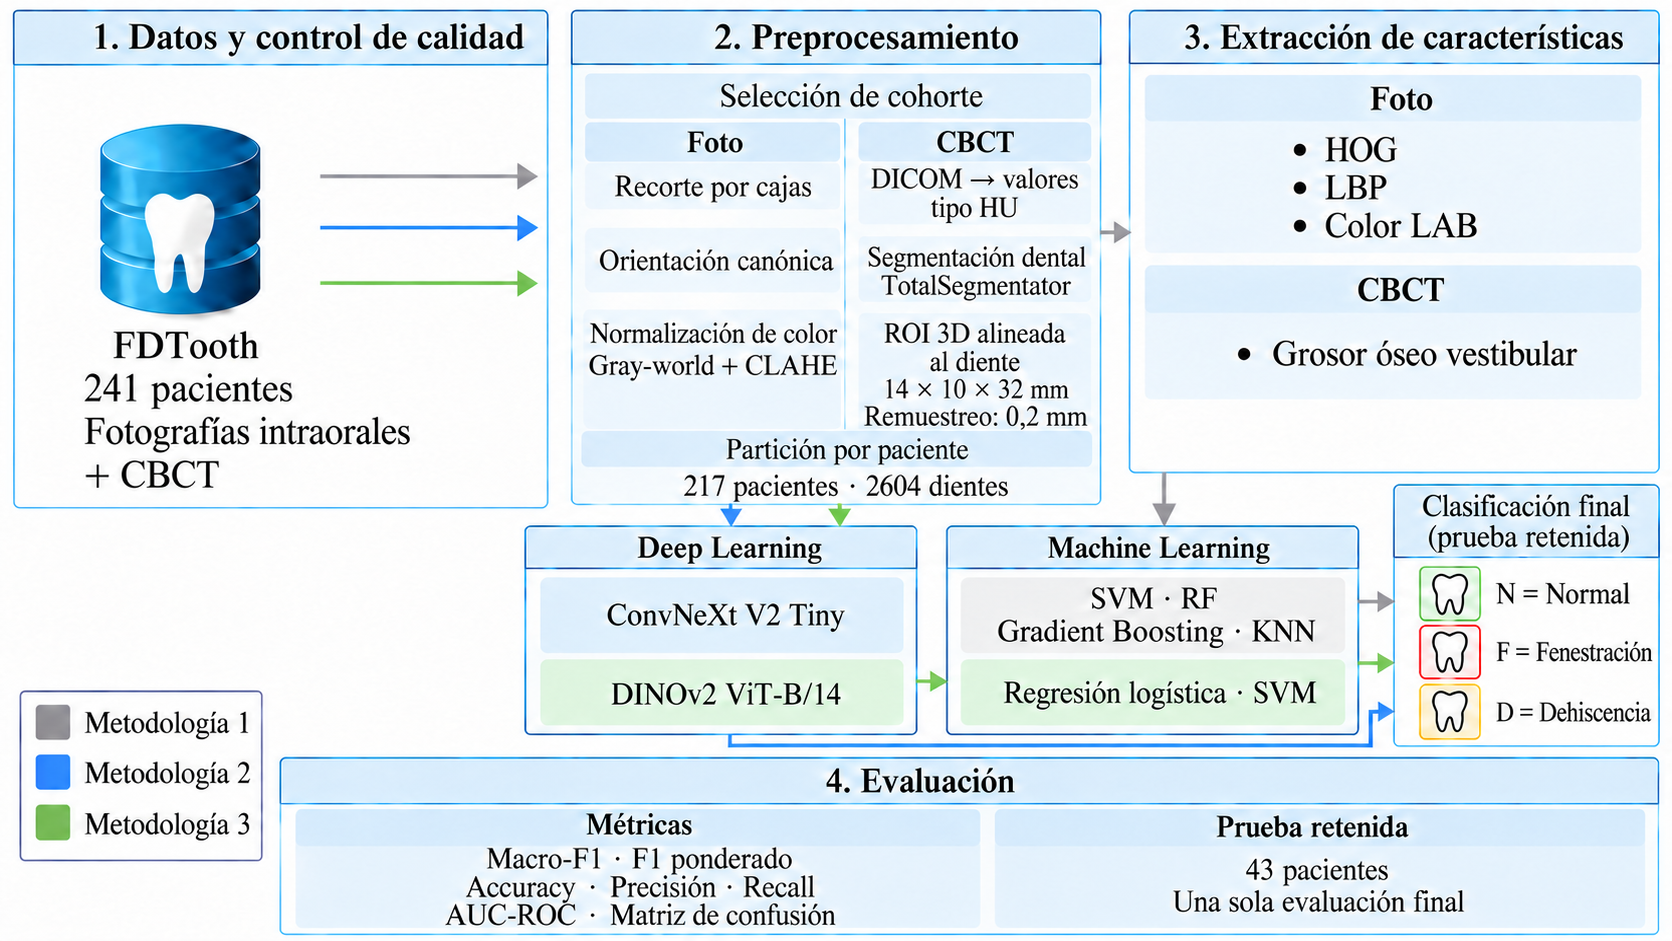
\includegraphics[width=\textwidth]{metodologia.png}
\caption{Metodología propuesta}
\label{fig:metodologia}
\end{figure}

\subsubsection{Desarrollo de la metodología}
% Fases según img/metodologia.png. Cada fase origina un PE, un OE y una HE.
\paragraph{Fase 1: Datos y control de calidad}
% Usar \dat{FDTooth}, \dat{CBCT}, \dat{fotografía intraoral} en el texto.
Por redactar.
\paragraph{Fase 2: Preprocesamiento}
% Foto: recorte por cajas, orientación canónica, Gray-world + CLAHE.
% CBCT: DICOM -> HU, TotalSegmentator, ROI 3D 14 x 10 x 32 mm a 0.2 mm.
% Partición por paciente: 217 pacientes, 2604 dientes.
Por redactar.
\paragraph{Fase 3: Extracción de características y modelado}
% M1: HOG, LBP, color LAB y grosor óseo vestibular + SVM, RF, GB, KNN.
% M2: ConvNeXt V2 Tiny. M3: DINOv2 ViT-B/14 + regresión logística y SVM.
Por redactar.
\paragraph{Fase 4: Evaluación}
% Macro-F1, F1 ponderado, Accuracy, Precisión, Recall, AUC-ROC y matriz de
% confusión; prueba retenida de 43 pacientes evaluada una sola vez.
Por redactar.

\subsubsection{Metodología para la medición de resultados}
El análisis de los resultados de la implementación se realizará mediante la
evaluación \ldots

% ======================= REFERENCIAS (APA 7) =========================
\clearpage
\seccionsinnumero{Referencias}
\nocite{*} % temporal: quitar cuando el texto ya tenga \textcite/\parencite
{\onehalfspacing
\printbibliography[heading=none]}

% ======================= ANEXOS =====================================
\clearpage
\seccionsinnumero{Anexos}
\noindent\textbf{Anexo 1: Matriz de Consistencia}

{\singlespacing\small
\begin{tabularx}{\textwidth}{|X|X|X|X|X|}
\hline
\textbf{Problemas} & \textbf{Objetivos} & \textbf{Hipótesis} &
\textbf{Variables e indicadores} & \textbf{Metodología} \\ \hline
PG: & OG: & HG: & VI: & Diseño: \\
PE1: & OE1: & HE1: & VD: & Tipo: \\
PE2: & OE2: & HE2: & Indicadores: & Enfoque: \\
PE3: & OE3: & HE3: & & \\
PE4: & OE4: & HE4: & & \\ \hline
\end{tabularx}}

\end{document}
